\documentclass{bredelebeamer}

%%%%%%%%%%%%%%%%%%%%%%%%%%%%%%%%%%%%%%%%%%%%%%%%

\title[Programación en MatLAB]{Introducción a la programación con MatLAB}
\subtitle{Módulo 10 - Álgebra matricial}

\author{Agustín - Andrés - Gabriel - Fernando\inst{1}}
\institute[UTN.BA]
{
  \inst{1}%
  Universidad Tecnológica Nacional\\
  Facultad Regional Buenos Aires
  }

\date{2018}

\subject{Taller de programación}

\logo{

\includegraphics[scale=0.15]{images/logo.png}
}

%%%%%%%%%%%%%%%%%%%%%%%%%%%%%%%%%%%%%%%%%%%%%%%%%%%%%%%%%%%%%%%%%%%%%
\begin{document}

\begin{frame}
  \titlepage 
\end{frame}

%%%%%%%%%%%%%%%%%%%%%%%%%%%%%%%%%%%%%%%%%%%%%%%%%%%%%%%%%%%%%%%%%%%%%

% Algebra matricial

%%%%%%%%%%%%%%%%%%%%%%%%%%%%%%%%%%%%%%%%%%%%%%%%%%%%%%%%%%%%%%%%%%%%%
\section{Algebra matricial}

\begin{frame}{Transpuesta}
\textbf{Operador transpuesta:} 
\begin{center}
Transpuesta\_A = A'
\end{center}
\begin{center}
Cambia las filas de una matriz en culumnas y las columnas en fila
\end{center}
Ej. Ejecutar las siguientes líneas. Obtener conclusiones.
\lstinputlisting[xleftmargin=.3\textwidth]{scripts/ej1.m}
\end{frame}

\begin{frame}{Producto punto}
\textbf{Producto escalar:}
\begin{center}
Vector\_resultante = \textbf{sum}(A\textbf{.*}B)
\end{center}
Ej. Ejecutar las siguientes líneas. Obtener conclusiones.
\lstinputlisting[xleftmargin=.3\textwidth]{scripts/ej2.m}
\end{frame}

\begin{frame}{Producto punto}
\begin{exampleblock}{Comando}
Ver comando: dot()
\end{exampleblock}
Ej. Ejecutar las siguientes líneas. Obtener conclusiones.
\lstinputlisting[xleftmargin=.3\textwidth]{scripts/ej3.m}
\end{frame}

\begin{frame}{Ejercicio práctico 15}
\begin{enumerate}
\item Use la función dot para encontrar el producto punto de los siguientes vectores:
\begin{itemize}
\item A = [1 2 3 4]
\item B = [12 20 15 7]
\end{itemize}
\item Encuentre el producto punto de A y B al sumar los productos arreglo de A y B (sum(A.*B))
\end{enumerate}
\end{frame}

\begin{frame}{Multiplicación matricial}
\textbf{Producto matricial:}
\begin{center}
Vector\_resultante = A*B
\end{center}
Ej. Ejecutar las siguientes líneas. Obtener conclusiones.
\lstinputlisting[xleftmargin=.3\textwidth]{scripts/ej4.m}
\end{frame}

\begin{frame}{Potencias de matrices}
\textbf{Elevar a la potencia N cada elemento de la matriz} \textbf{.\^}
\begin{center}
Vector\_resultante = A.\^N
\end{center}
Ej. Ejecutar las siguientes líneas. Obtener conclusiones.
\lstinputlisting[xleftmargin=.3\textwidth]{scripts/ej5.m}
\end{frame}

\begin{frame}{Inversión de matriz}
\begin{exampleblock}{Comando}
Ver comando: inv()
\end{exampleblock}
Ej. Ejecutar las siguientes líneas. Obtener conclusiones.
\lstinputlisting[xleftmargin=.3\textwidth]{scripts/ej6.m}
\end{frame}

\begin{frame}{Determinantes}
\begin{exampleblock}{Comando}
Ver comando: det()
\end{exampleblock}
Ej. Ejecutar las siguientes líneas. Obtener conclusiones.
\lstinputlisting[xleftmargin=.3\textwidth]{scripts/ej7.m}
\end{frame}

\begin{frame}{Inversión de matriz}
Ej. Ejecutar las siguientes líneas. Obtener conclusiones.
\lstinputlisting[xleftmargin=.3\textwidth]{scripts/ej8.m}
\end{frame}

\begin{frame}{Inversión de matriz}
\begin{columns}
\begin{column}{0.5\textwidth}
\begin{center}
\LARGE det(A)
\end{center}
\end{column}
\begin{column}{0.5\textwidth}
\begin{center}

\includegraphics[scale=0.25]{images/img40.png}
\end{center}
\end{column}
\end{columns}
\end{frame}

\begin{frame}{Inversión de matriz}
\begin{columns}
\begin{column}{0.5\textwidth}
\begin{center}
\LARGE det(A)
\end{center}
\end{column}
\begin{column}{0.5\textwidth}
\begin{center}

\includegraphics[scale=0.25]{images/img40.png}
\end{center}
\end{column}
\end{columns}
\begin{alertblock}{Algebra!}
det(A) = 0 \textbf{entonces} matriz singular. No existe la inversa!
\end{alertblock}
\end{frame}

\begin{frame}{Ejercicio práctico 16}
\begin{enumerate}
\item Encuentre el inverso de las siguientes matrices mágicas, tanto con la función inv como al elevar la matriz a la potencia -1:
\begin{itemize}
\item magic(3)
\item magic(4)
\item magic(5)
\end{itemize}
\item Encuentre el determinante de cada una de las matrices de la parte 1
\end{enumerate}
\end{frame}

\begin{frame}{Matrices especiales: unos y ceros}
\begin{exampleblock}{Comando}
Ver comando: ones()
\end{exampleblock}
\begin{columns}
\begin{column}{0.5\textwidth}
Ej. Ejecutar las siguientes líneas. Obtener conclusiones.
\lstinputlisting[xleftmargin=.2\textwidth]{scripts/ej9.m}
\end{column}
\begin{column}{0.5\textwidth}
\begin{center}
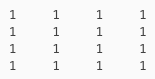
\includegraphics[scale=0.5]{images/pantalla1.png}
\end{center}
\end{column}
\end{columns}
\end{frame}

\begin{frame}{Matrices especiales: unos y ceros}
\begin{exampleblock}{Comando}
Ver comando: ones()
\end{exampleblock}
\begin{columns}
\begin{column}{0.5\textwidth}
Ej. Ejecutar las siguientes líneas. Obtener conclusiones.
\lstinputlisting[xleftmargin=.2\textwidth]{scripts/ej9.m}
\end{column}
\begin{column}{0.5\textwidth}
\begin{center}
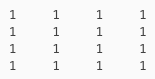
\includegraphics[scale=0.5]{images/pantalla1.png}
\end{center}
\end{column}
\end{columns}
\begin{exampleblock}{Comando}
Ver comando: zeros()
\end{exampleblock}
\begin{columns}
\begin{column}{0.5\textwidth}
Ej. Ejecutar las siguientes líneas. Obtener conclusiones.
\lstinputlisting[xleftmargin=.2\textwidth]{scripts/ej10.m}
\end{column}
\begin{column}{0.5\textwidth}
\begin{center}
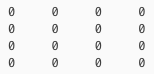
\includegraphics[scale=0.5]{images/pantalla2.png}
\end{center}
\end{column}
\end{columns}
\end{frame}

\begin{frame}{Matrices especiales: Matriz identidad}
\begin{exampleblock}{Comando}
Ver comando: eye()
\end{exampleblock}
\begin{columns}
\begin{column}{0.5\textwidth}
Ej. Ejecutar las siguientes líneas. Obtener conclusiones.
\lstinputlisting[xleftmargin=.2\textwidth]{scripts/ej11.m}
\end{column}
\begin{column}{0.5\textwidth}
\begin{center}
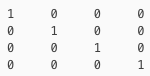
\includegraphics[scale=0.5]{images/pantalla3.png}
\end{center}
\end{column}
\end{columns}
\end{frame}

\begin{frame}{Ejercicio práctico 17}
\begin{center}
\begin{itemize}
\item Considere la siguiente matriz: A = [1 2 3 ; 2 4 6 ; 3 6 9]. Calcule el determinante de A. Es inversible?
\end{itemize}
\end{center}
\begin{block}{Recordar}
Si el $det(A) \neq 0$, entonces la matriz es inversible.
\end{block}
\end{frame}

\begin{frame}{Ejercicio práctico 17}
\begin{center}

\includegraphics[scale=0.35]{images/img43.png}
\end{center}
\end{frame}

\begin{frame}{Ejercicio práctico 17}
\begin{center}
\LARGE inv(A)
\end{center}
\end{frame}

\begin{frame}{Ejercicio práctico 17}
\textbf{Resupuesta:}
\begin{block}{Tener en cuenta}
Si el $det(A)\neq 0$, entonces las columnas de A son linealmente independientes y, por lo tanto, A es inversible.
\end{block}
\end{frame}

\begin{frame}{Ejercicio práctico 17}
\textbf{Resupuesta:}
\begin{block}{Tener en cuenta}
Si el $det(A)\neq 0$, entonces las columnas de A son linealmente independientes y, por lo tanto, A es inversible.
\end{block}
\begin{center}
Matriz propuesta\\
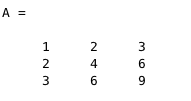
\includegraphics[scale=0.5]{images/img44.png}
\end{center}
\end{frame}

\begin{frame}{Ejercicio práctico 17}
\begin{columns}
\begin{column}{0.6\textwidth}
\begin{center}
\textbf{Eran todas linealmente dependientes }
\end{center}
\end{column}
\begin{column}{0.3\textwidth}
\begin{center}

\includegraphics[scale=0.3]{images/img45.png}
\end{center}
\end{column}
\end{columns}
\begin{center}

\includegraphics[scale=0.6]{images/img42.png}
\end{center}
\end{frame}

\end{document}
